\documentclass[a5paper]{article}
\usepackage[a5paper, top=8mm, bottom=8mm, left=8mm, right=8mm]{geometry}

\usepackage{polyglossia}
\setdefaultlanguage[babelshorthands=true]{russian}

\usepackage{fontspec}
\setmainfont{FreeSerif}
\newfontfamily{\russianfonttt}[Scale=0.7]{DejaVuSansMono}

\usepackage[font=scriptsize]{caption}

\usepackage{amsmath}
\usepackage{amssymb,amsfonts,textcomp}
\usepackage{color}
\usepackage{array}
\usepackage{hhline}
\usepackage{cite}
\usepackage{textcomp}

\usepackage[hang,multiple]{footmisc}
\renewcommand{\footnotelayout}{\raggedright}

\PassOptionsToPackage{hyphens}{url}\usepackage[xetex,linktocpage=true,plainpages=false,pdfpagelabels=false]{hyperref}
\hypersetup{colorlinks=true, linkcolor=blue, citecolor=blue, filecolor=blue, urlcolor=blue, pdftitle=1, pdfauthor=, pdfsubject=, pdfkeywords=}

\newlength\Colsep
\setlength\Colsep{10pt}

\usepackage{tabu}

\usepackage{graphicx}
\usepackage{indentfirst}
\usepackage{multirow}
\usepackage{subfig}
\usepackage{footnote}
\usepackage{minted}

\newcommand{\todo}[1] {
\begin{center}\textcolor{red}{TODO: #1}\end{center}
}

\sloppy
\pagestyle{plain}

\title{Объектно-ориентированное программирование на C\#, введение}
\author{Юрий Литвинов\\\small{yurii.litvinov@gmail.com}}

\date{15.02.2019г}

\begin{document}

\maketitle
\thispagestyle{empty}

\section{Про что этот курс}

Этот семестр --- про объектно-ориентированное программирование и связанные вещи, а также технологические аспекты разработки ПО. То есть, в курсе не будет (или почти не будет) новых алгоритмов, зато будет много новых концепций и конкретных технологий, которые могут пригодиться на практике. Начнём мы с ликвидации безграмотности по языку C\#. Именно на примере этого языка будут объясняться основные концепции объектно-ориентированного программирования и вообще вещи, свойственные современным объектно-ориентированным языкам, но курс ни в коем случае не про C\#, знания могут быть легко распространены на C++ или Java. Дальше будет про ООП (основные понятия: объекты, классы, абстракция-инкапсуляция-наследование-полиморфизм и т.д.), про генерики, про события, лямбды, про реализацию пользовательских интерфейсов. Также будут затронуты и технологические аспекты: модульное тестирование, практика code review, визуальное моделирование на языке UML.

Домашек будет немного меньше, чем в первом семестре, но они будут объёмнее. Пар будет только одна в неделю, так что особо углубляться в технические детали будет некогда, придётся больше гуглить и разбираться самостоятельно. В середине семестра будет контрольная, в конце семестра будет зачётная работа. Как обычно, надо сдать все домашки, написать все задачи контрольной и зачётной работ. Будут доклады про разные технологии вокруг .NET, успешным докладом, как обычно, можно закрыть одну домашку. Домашки надо будет сдавать пуллреквестом в свой репозиторий на GitHub, как в прошлом семестре, надо записаться на этот семестр в HwProj (\url{http://hwproj.me/courses/34}) и, возможно, он позволит отмечать сданные домашки там. Если нет, то надо писать мне на почту, что домашка готова к проверке.

В принципе, в этом курсе всё будет рассказываться с нуля, но если то, что рассказывалось на лекциях, заинтересовало и хочется почитать поподробнее про то, как всё работает, рекомендую книгу Jeffrey Richter. CLR via C\#. Это фактически must read для любого профессионального .NET-программиста, хотя может быть сложновата на первом курсе. Может, к середине-концу семестра имеет смысл начать её читать. Есть ещё много разных книжек по C\#, так что если что-то на парах непонятно, можно посмотреть там, но все они, как говорят, так себе (впрочем, я не читал). Из таких книжек C\# in Depth в интернетах хвалят. Читать лучше на английском, но если совсем никак, всё это есть в русском переводе. Ещё есть несколько годных блогов по .NET, но рекомендовать могу, пожалуй, только официальный блог Microsoft.

\section{Язык C\#, введение}

Язык программирования С\# был разработан компанией Microsoft как основной язык программирования для платформы .NET, первая версия была представлена публике в 2002 году. Впоследствии он был стандартизован ECMA (ECMA-334) и ISO (ISO/IEC 23270:2006), то есть в данный момент является международным стандартом. Последняя на данный момент версия языка, C\# 7.3, опубликована 7 мая 2018 года. Язык создавался как простой в использовании объектно-ориентированный язык общего назначения, с сильной типизацией. Используется в основном для написания прикладного ПО (включая настольные приложения, веб-приложения, он же используется для программирования под Windows Phone мобильных приложений). Всякие драйвера или системное ПО типа СУБД лучше писать на C++ (как правило, работать будет побыстрее, хотя это вопрос спорный в силу наличия в .NET развитых средств Just-in-time-компиляции). Программы, с которыми будут работать обычные пользователи --- типа банковских систем, программ складского учёта, информационных систем предприятия и т.д. вполне удобно писать на C\#, что очень многие и делают (язык занимает 7-е место в индексе TIOBE, \url{http://www.tiobe.com/index.php/content/paperinfo/tpci/index.html}). Ближайший конкурент C\# --- это, скорее, Java, языки довольно похожи (поначалу были очень похожи, но теперь их пути более-менее разошлись). Принципиальная разница в том, что Java ориентирована на кроссплатформенность, C\# создавался Microsoft для работы с их стеком технологий, однако же сейчас программы на C\# прекрасно работают практически на чём угодно, есть реализация .NET-машины с открытым исходным кодом Mono, есть .NET Core, есть открытая реализация почти всего .NET до версии 4.5 (вот только без WPF и только с частичной поддержкой WCF). В общем, весь код, что мы будем писать в этом семестре должен прекрасно работать под линуксом и под маком. В основном разработка на C\# ведётся в Microsoft Visual Studio (Community Edition бесплатна и её вполне достаточно для всех практических целей), набирает популярность Rider IDE от JetBrains (\url{https://www.jetbrains.com/rider/}, он кроссплатформенный и работает на чём угодно, к тому же бесплатный для студентов. Есть ещё MonoDevelop, на котором всё тоже можно делать, с большей или меньшей степенью удобства, есть Visual Studio Code, которая работает под линуксом и маком, но это скорее текстовый редактор, чем полноценная IDE. Есть ещё куча текстовых редакторов, таких как Atom, Sublime, они тоже подойдут, но очень многое они не умеют.

C\# называется ``си шарп'' примерно по тем же причинам, почему С++ называется С++ --- диез в музыке указывает на то, что ноту следует играть на полтона выше, так же как ++ --- оператор инкремента. C\# можно рассматривать как развитие C++, при этом C\# имеет ряд особенностей, которыми он радикально отличается от C++. Самая главная особенность, пожалуй, это использование виртуальной машины. Как происходит исполнение программы, написанной на C++ --- исходный код компилируется сразу в исполнимый код, который линкуется в исполняемый файл, который может быть загружен в память и исполнен той операционной системой, для которой он предназначается. Другая операционная система скомпилированную программу исполнить не сможет. В C\# принцип работы совсем другой, C\# --- один из языков, совместимых с так называемой Common Language Infrastructure. Его исходный код компилируется в последовательность команд некоей абстрактной машины (в т.н. байт-код .NET), которая потом интерпретируется специальным приложением --- дотнет-машиной. Дотнет-машина должна быть реализована для каждой операционной системы, на которой нужно запускать приложения на C\#, зато, поскольку система команд машины стандартизована (это тоже международный стандарт, предложенный Майкрософт и реализованный в .NET и Mono), это теоретически позволяет исполнять C\#-приложение под любой операционной системой, для которой есть дотнет-машина (такой принцип называется ``скомпилированное однажды, запускается везде'' (compile once, run anywhere), в отличие от переносимости на уровне исходных кодов ``write once, run anywhere''). Схематично такой подход можно изобразить так:

\begin{center}
	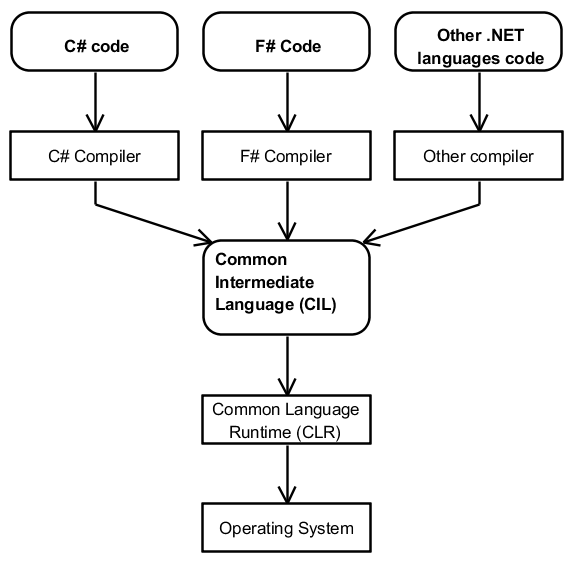
\includegraphics[width=0.6\textwidth]{cli.png}
\end{center}

В реальности, конечно, не всё так радостно, поскольку оригинальная реализация дотнет-машины и библиотек времени выполнения от Microsoft по большей части проприетарна и ни на чём, кроме ОС Windows, не работает. Относительно недавно Microsoft выложил исходники некоторых частей дотнета (в том числе, исходники компилятора C\# и основных библиотек), на это всё можно посмотреть на гитхабе (\url{https://github.com/dotnet}). Однако CLI (собственно, стандартизация байт-кода, дотнет-машины и библиотек поддержки) создавалась не для обеспечения переносимости, (которая была не очень-то выгодна Microsoft), а для того, чтобы иметь несколько языков программирования, работающих с одними библиотеками в одинаковой среде. Кроме C\#, в байт-коды дотнет-машины компилируется Visual Basic, J\# (ныне покойный), F\#, ещё куча всяких языков, созданных уже не Microsoft (например, Delphi с версии 8 умел компилироваться в байт-код .NET) --- наличие единого байт-кода и виртуальной машины, его исполняющей, фактически избавляет от необходимости писать часть компилятора, относящуюся к низкоуровневой оптимизации и генерации машинного кода, уменьшая работу по созданию компилятора минимум на треть, и заодно делая все языки бинарно совместимыми совершенно даром. Бинарная совместимость означает, что код, написанный на одном языке (функция, процедура, класс, и т.д.), может быть безболезненно использован в программах, написанных на другом языке. Это очень удобно, поскольку ``отвязывает'' библиотеки от языка реализации, можно писать библиотеки на чём угодно, и легко ими пользоваться, и даже в одном проекте можно писать код на разных языках. 

Кроме того, дотнет-машина может следить за выполнением программы более строго, чем операционная система --- за выполнением ``native''-программы, например, сразу же обнаружить попытку чтения или записи в чужую область памяти, выход за границы массива и т.д. Кроме того, переменные сами инициализируются, исполняемая программа имеет в себе кучу отладочной информации, и вообще, жизнь программиста делается более простой и приятной.

За такое удобство приходится платить падением скорости работы программы --- ведь интерпретировать инструкцию гораздо дороже, чем просто исполнить её на процессоре. Однако с этим научились бороться, с помощью техники, называемой Just-In-Time-компиляцией. JIT-компиляция --- это когда последовательность инструкций байт-кода переводится в машинный код прямо в процессе выполнения программы, после чего запоминается для последующего использования. При этом дотнет-машина может использовать для оптимизации информацию, недоступную ``статическим'' компиляторам --- например, в процессе работы смотреть, какая функция вызывается чаще, и делать для неё инлайн-подстановку. Так что в целом, хоть хорошо написанные программы на С++, скорее всего, будут работать быстрее, дотнет-машина может выигрывать в производительности у плохо написанных программ на С++, и, поскольку время работы программиста сейчас гораздо дороже, чем время работы программы (как правило), приложения всё больше пишут на C\# (ну или Яве).

Следует отметить, что виртуальную машину в качестве среды выполнения использует далеко не только C\# (ну, в смысле, языки CLI, их много) --- программы на Яве или Котлине тоже исполняются джава-машиной, идея виртуальной машины была предложена ещё Виртом для языка Паскаль (в 70-х годах 20-го века, так что это не суперновая технология). Причём в код Java-машины тоже можно компилировать не одну только Java --- есть ещё языки, типа Скалы, и Котлина, ориентирующиеся на Java-машину как среду выполнения, или Ада --- которая имеет компилятор в байт-код Java помимо нативного кода.

Следующим важным отличием C\# от С++ является сборка мусора. В С++ надо было следить за выделением памяти --- память, выделенную в куче, надо было освобождать вручную. В C\# выделять память надо, а освобождать --- нет, это сделает сама дотнет-машина, точнее, сборщик мусора (garbage collector). Дотнет-машина следит за тем, на какие области памяти ссылается программа, и если есть выделенная область памяти, на которую не ссылается больше никто, она её удалит. Опять же, это не особенность дотнет, джава-машина поступает так же, а сама идея сборки мусора предлагалась ещё в лиспе, в 1959. Концептуально сборка мусора работает так: все области памяти помечаются как ``ненужные'', потом все переменные на стеке вызовов помечаются как ``нужные'', потом все области памяти, на которые указывают переменные на стеке вызовов или их поля помечаются как ``нужные'', потом все области памяти, на которые указывают ``нужные'' области памяти, помечаются как нужные и т.д., пока не останется указателей, на которые мы ещё не смотрели. Те области памяти, которые остались помечены как ``ненужные'', очищаются (это алгоритм mark-and-sweep). Картинка из википедии, поясняющая суть:

\begin{center}
	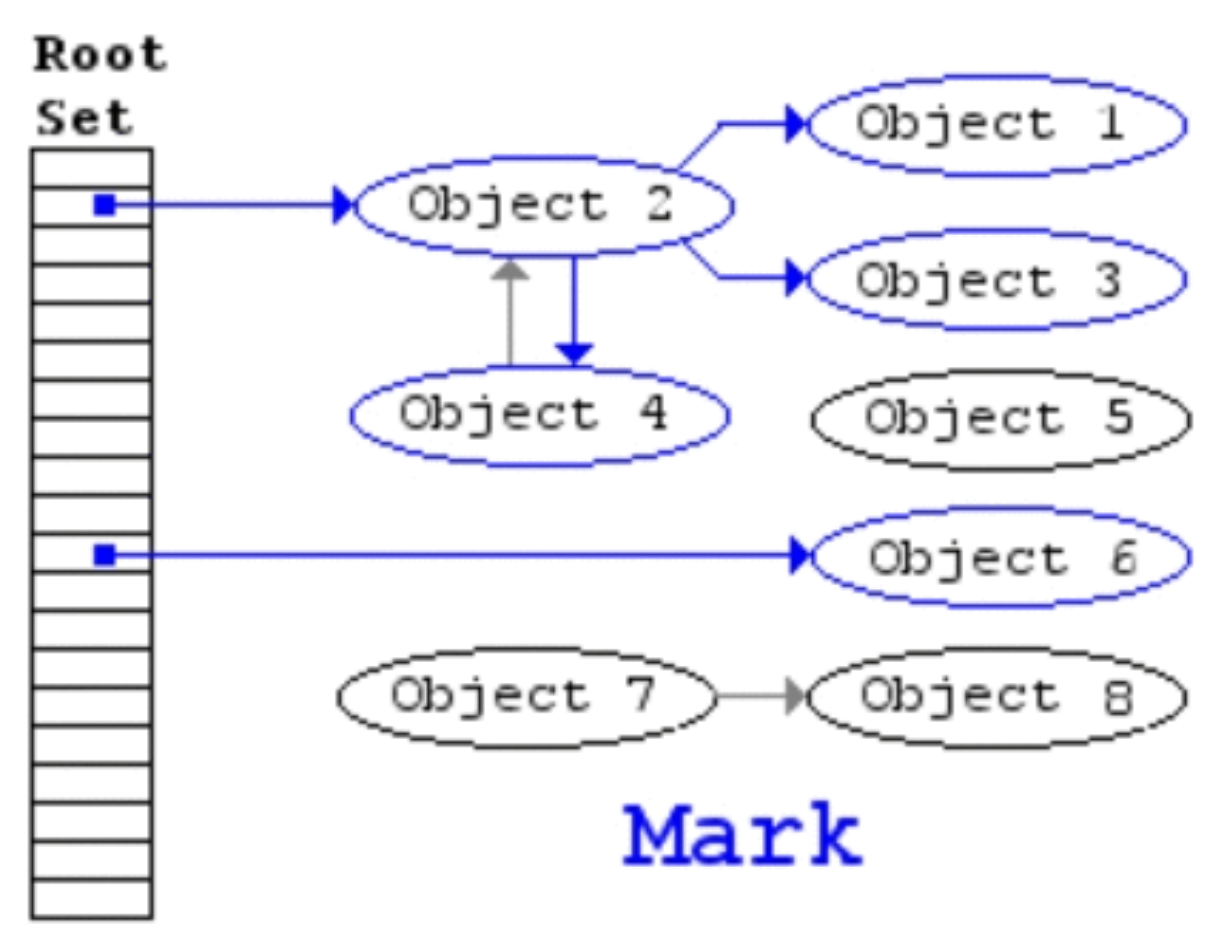
\includegraphics[width=0.4\textwidth]{markAndSweep.png}
\end{center}

В реальности используются более сложные алгоритмы, поскольку, во-первых, сборка мусора --- это вычислительно сложная операция (средняя игра занимает в памяти до 8Гб, ходить по ней всей фактически поиском в ширину сложновато), во-вторых, требуется остановка приложения (иначе если память будет выделена или освобождена в процессе работы сборщика мусора, всё умрёт). Так что используются поколения, параллельная сборка мусора, оптимизации типа Large Object Heap и т.д., про что потом будет доклад, по идее. Сейчас важно понимать, что про delete в C\# можно забыть, как про страшный сон. Естественно, организовать себе утечку памяти можно даже в C\#, но это гораздо сложнее сделать случайно, для этого даже потребуется некоторое продвинутое знание языка. Что интересно, что благодаря тому, что выделение памяти выполняется виртуальной машиной из заранее выделенного пула памяти, причём это делается за константное время, программа, активно использующая кучу, на C\# может работать быстрее, чем на C++ (впрочем, современные компиляторы C++ используют оптимизации, похожие на то, что делается в C\#, так что кто победит трудно сказать заранее).

\section{Технические детали}

Собственно, традиционная программа ``Hello, world'':

\begin{minted}{csharp}
using System;

namespace HelloWorld
{
    class Program
    {
        static void Main(string[] args)
        {
            Console.WriteLine("Hello, world!");
        }
    }
}
\end{minted}

Что мы тут видим: во-первых, работающая программа на C\#, как и на любом другом объектно-ориентированном языке, представляет собой набор объектов, взаимодействующих друг с другом через чётко определённые интерфейсы посылкой и приёмом сообщений. Тип объекта --- это класс, т.е. класс описывает структуру и поведение объектов. Код программы на C\# представляет собой набор классов, классы организованы в нэймспейсы, свободных функций (не методов класса) в C\#, в отличие от C++, не бывает вообще. Что такое нэймспейс, вы, наверное, помните из С++, но если что, это такое средство группировки --- в одном нэймспейсе лежат связанные логически классы (ну, и другие типы), неймспейсы могут быть вложенными, позволяя создавать такую иерархическую структуру. Кстати, разделения на хедеры и cpp-шники в C\# нет, всё, что относится к одному классу, пишется в одном файле, с расширением .cs. Есть, правда, возможность определять класс в нескольких разных файлах, через partial-классы, но это нужно для некоторых специальных целей, про которые потом. Считается хорошим тоном поддерживать соответствие ``один файл --- один класс''. Так вот, каждый класс относится к некоторому неймспейсу, неймспейс можно и не писать, тогда класс будет считаться принадлежащим нэймспейсу по умолчанию, но это дурной тон. Одноимённые классы из разных неймспейсов можно различить, указывая квалифицированное имя класса: <имя пакета>.<имя класса>. Всё это на самом деле очень похоже на пространства имён C++. Кроме пакета, есть ещё понятие ``сборка'' (assembly) --- это отдельный проект, кусок кода, который собирается в отдельный .exe или .dll-файл. Один неймспейс может определяться в разных сборках, и одна сборка может иметь много неймспейсов, но тем не менее, сборки тоже работают как некое средство группировки, потому что позволяют управлять видимостью классов друг другу --- можно сделать класс видимым только внутри своей сборки, а можно сделать его видимым и в других сборках тоже (типа интерфейса сборки). Вообще, создавать отдельные библиотеки и использовать их в проекте очень легко, в отличие от C++, так что приложение на C\# (ну или вообще любом дотнет-языке), как правило, состоит из большего числа отдельно собираемых модулей, чем С++. Кстати, подключение неймспейса делается с помощью ключевого слова using, так что using System --- это подключение неймспейса System, ну, почти как в С++. Разве что в C++ было отдельно \#include и отдельно using namespace, здесь using --- это аналог using namespace, а аналога \#include в программе вообще нет. Видны все public-классы всех сборок, подключённых к данному проекту, во всех файлах проекта, а классы проекта видны в других файлах проекта вообще всегда, что по сравнению с C++ сказочно удобно.

Дальше мы видим объявление класса Program. Внутри фигурных скобочек находятся объявления полей, методов и свойств класса, вложенных классов, перечислений и т.д. В нашем случае в классе есть только метод Main, он static --- то есть он является методом класса, в противоположность обычным методам, которые относятся к конкретному объекту. Методы класса не используют данные, хранящиеся в объекте, так что наличие объекта им не нужно для работы. Это самое близкое, что есть в C\# к обычным сишным функциям, которыми вы пользовались в прошлом семестре. Он имеет тип возвращаемого значения void, то есть, как и в C++, это означает, что он не возвращает ничего. Заметим, что в отличие от С++ C\#-овая ``функция'' Main код возврата сама не должна возвращать. Эта функция принимает один параметр --- массив строк (то есть, объектов класса String, представляющих строки, про сишные char*, развлечения с указателями и всякие соглашения типа того, что строка кончается на \\0, можно забыть, как страшный сон, то есть внутри оно всё так и есть, но хорошо скрыто, что, в частности, является преимуществом объектно-ориентированного программирования). Аналог C\#-ового String – С++-ный std::string. Массивы в C\# тоже не так просты, как в С++, а представляют собой объекты, с полями и методами, например, у них есть свойство Length, которое содержит длину массива.

Дальше стоит вызов метода WriteLine класса Console. Он, как и следовало ожидать, печатает на консоль строку и переводит строку. У Console есть ещё много всяких полезных методов, например, Beep, и ещё больше всяких свойств, типа ForegroundColor (и BackgroundColor), и Title. Есть ещё метод Write, который делает то же, что и WriteLine, но не переводит строку. Заметьте, WriteLine может выводить всё без всякой форматной строки, но если нужна форматная строка, тоже ок: \mintinline{csharp}|Console.WriteLine("Hello, {0}!", "world");|. Заметьте, никаких форматных спецификаторов не надо, C\# сам догадывается о типе выводимых параметров.

Синтаксис тел методов весьма похож на C++, так что скорее всего получится просто сесть и начать писать код так, будто бы это был С++. Например, цикл for:

\begin{minted}{csharp}
for (int i = 0; i < 300; ++i)
{
    Console.WriteLine("Hello, world!");
}
\end{minted}

или так: 

\begin{minted}{csharp}
for (var i = 0; i < 300; ++i)
{
    Console.WriteLine("Hello, world!");
}
\end{minted}

Тут показана интересная фича C\# --- частичный вывод типов. i инициализируется интовой константой 0, так что компилятор знает, что тип переменной i должен быть интом (иначе типы не сойдутся), так что это можно не указывать и писать вместо имени типа var. Тут, правда, есть идеологический спор по поводу того, как часто надо использовать var. Некоторые говорят, что var использовать нельзя, потому что явные аннотации типов накладывают дополнительные ограничения на программу, и тем самым уменьшают вероятность ошибок и делают программу гораздо более читабельной. Некоторые говорят, что var надо использовать всегда, поскольку информация о типе избыточна и до тех пор, пока компилятор может вывести тип, не несёт семантической нагрузки, к тому же короткое var в коде выглядит гораздо лучше, чем какое-нибудь System.Collections.Generic.Dictionary<string, int>, так что использование var делает программу гораздо более читабельной. Некоторые занимают промежуточную позицию и предпочитают использовать var только чтобы не писать длинных имён типов. Лично я люблю var, и предлагаю вам им активно пользоваться, хотя бы в тех случаях, когда тип переменной очевиден из правой части присваивания (например, var str = new String(``s''); ). Кстати, в среде даже опытных программистов распространена ересь, что var ломает строгую типизацию, делая тип переменной ``неопределённым'' --- это неправда, тип переменной в любом случае точно известен во время компиляции, ломает типизацию другая штука --- dynamic, но про неё лучше забудьте прямо сейчас.

Функции задаются, например, так:

\begin{minted}{csharp}
private static int Factorial(int n)
{
    if (n == 1)
    {
        return 1;
    }

    return n * Factorial(n - 1);
}
\end{minted}

--- это нужно писать в классе Program на том же уровне, что и функция Main. Использовать из функции Main, например, так:

\begin{minted}{csharp}
Console.WriteLine(Factorial(4));
\end{minted}

Кстати, компилятор многопроходный, поэтому ему плевать, выше или ниже функции Main описана наша функция.

В современном C\# функции, тело которых состоит из одной строчки, можно писать вообще в одну строку, без фигурных скобок, вот так:

\begin{minted}{csharp}
private static int Factorial(int n) => n <= 1 ? 1 : n * Factorial(n - 1);
\end{minted}

Это назыввается Expression-bodied method, и когда мы дойдём до рассказа про лямбда-функции, будет понятно, почему оно так выглядит. Это на самом деле синтаксический сахар для того, чтобы писать программы кратко и красиво (хотя такой синтаксис может быть непривычен сишникам).

Обратите внимание на некоторые особенности местного стайлгайда. Вообще, стайлгайд тут не как в С++, где пишут кто как умеет, а определяется исходниками от Майкрософт, так что довольно строгий (ну, вариации есть, но некоторые правила вообще общеприняты). Имена методов и свойств пишутся всегда с заглавной, имена полей всегда со строчной. Тела составных операторов, типа if-ов, считается хорошим тоном всегда оборачивать в фигурные скобки, но этому следуют не всегда. То же касается отделения закрывающей фигурной скобки пустой строкой от кода ниже. Некоторые правила стайлгайда Visual Studio применяет автоматически и без спроса, так что не удивляйтесь, если вы пишете как обычно, а получается всё равно хорошо. Есть даже плагин к Visual Studio (и отдельный анализатор, подключаемый к проекту), который выдаёт предупреждения при нарушении общепринятого стайлгайда, \url{https://github.com/DotNetAnalyzers/StyleCopAnalyzers}. Очень рекомендую, хотя часть предупреждений придётся отключить, особенно поначалу (например, подписывать сборки мы не будем).

\section{Типы данных}

С типами данных в C\# ситуация несколько отличается от C++. Во-первых, размеры элементарных типов данных стандартизованы, так что если число байт, выделяемых под int в C++ зависело от реализации, то в C\# это ровно 32 байта, даже если мы запускаем программу на микроволновке с 16-битным процессором. Во-вторых, что даже более важно, каждый тип данных в C\# --- это класс, даже int наследуется от класса System.Object и имеет методы. Хорошая новость в том, что это на прикладных программистов особо не влияет (даже делает более удобной работу с элементарными типами) --- int-ы всё так же располагаются на стеке вызовов и копируются при присваивании. Подробности про это на следующей паре.

Каждый элементарный тип имеет своё ключевое слово, как в С++, и ещё имя типа, объявленное в библиотеке Base Class Library (неймспейс System), которое его синоним. Так что string и System.String --- это одно и то же.

У каждого типа есть значение по умолчанию, которым его переменные инициализируются сразу при объявлении. Неинициализированных переменных, с которыми приходилось бороться в C++, в C\# просто не бывает (хотя компилятор будет ругаться, если, например, пытаться передать как параметр локальную переменную, которой не было присвоено значение). Вообще, компилятор внимательно анализирует поток данных и выдаёт ошибку, если ему кажется, что что-то не так.

У типов-синонимов есть полезные статические методы, которые есть и у, мм, ключевых слов, им соответствующих. Например, как преобразовать строку в число:

\begin{minted}{csharp}
var inputString = Console.ReadLine();
int number = Int32.Parse(inputString);
\end{minted}

Это то же самое, что и

\begin{minted}{csharp}
var inputString = Console.ReadLine();
int number = int.Parse(inputString);
\end{minted}

В общем-то, с ООП все должны быть хотя бы примерно знакомы, но для программистов на чистом C это выглядит диковато.

Массивы:

\begin{minted}{csharp}
int[] a = new int[10];
\end{minted}

или

\begin{minted}{csharp}
var a = new int[10];

for (var i = 0; i < a.Length; ++i)
{
    a[i] = i;
}
\end{minted}

Тут всё как обычно, единственное, что массивы всегда размещаются на куче (то есть без ключевого слова new создать массив нельзя), квадратные скобочки пишутся после типа, а не после переменной, как в C++, и главное, массив --- это объект (имеющий, например, свойство Length, в котором хранится его длина, поэтому передавать длину вместе с массивом больше не надо). Для тех, кто в курсе, очевидна аналогия с std::vector.

Многомерные массивы:

\begin{minted}{csharp}
int[,] numbers = new int[3, 3];
numbers[1,2] = 2;
 
int[,] numbers2 = new int[3, 3] { {2, 3, 2}, {1, 2, 6}, {2, 4, 5} };
\end{minted}

Обратите внимание, что C\# поддерживает именно многомерные массивы, а не массивы массивов, как в C++. Массивы массивов тоже никто не запрещает:

\begin{minted}{csharp}
int[][] a = new int[3][];
a[1][2] = 0;
\end{minted}

--- так программа упадёт (угадайте почему), а вот так будет работать:

\begin{minted}{csharp}
int[][] a = new int[3][];
for (int i = 0; i < 3; ++i)
{
    a[i] = new int[3];
}

a[1][2] = 0;
\end{minted}

Структуры:

\begin{minted}{csharp}
struct Point
{
    public int x;
    public int y;
}
\end{minted}

Обратите внимание, что видимость по умолчанию у полей структуры такая же, как и у полей класса --- private, так что приходится писать public, чтобы они были доступны извне. А ещё в отличие от С++ писать модификатор видимости надо перед каждым полем и методом (ну, необязательно, но тогда видимость будет по умолчанию, и хорошим тоном считается модификатор видимости писать, даже если умолчание нас устраивает). Про всё это будет подробнее на следующей паре, структуры не так просты, как кажутся, но использовать их можно так же, как в C++.

Есть типы-перечисления:

\begin{minted}{csharp}
enum SomeEnum
{
    red,
    green,
    blue
}
\end{minted}

Использование:

\begin{minted}{csharp}
SomeEnum a = SomeEnum.blue;
\end{minted}

или так:

\begin{minted}{csharp}
var a = SomeEnum.blue;
\end{minted}

Обратите внимание, что имя енума должно предшествовать имени значения всегда, енум образует что-то вроде неймспейса для своих значений (как enum class в C++).

Константы задаются с помощью ключевого слова const, как и в С++ (но не как в Яве, где для этого есть ключевое слово final).

Всякие математические штуки находятся в классе Math неймспейса System. Например, Math.Cos(1); --- раз свободных функций в языке нет, функции на самом деле не функции, а статические методы. Хорошая новость в том, что есть using static, так что префикс Math можно не писать (особенно, если погуглить, что такое using static, и начать его использовать).

\section{Инструменты разработки}

Есть бесплатная Visual Studio Community 2017, которую можно скачать с \url{https://www.visualstudio.com/}, есть бесплатный для студентов Rider, который работает и под виндой, и под линуксом, и под маком (правда, пока не умеет дизайнить формочки в приложениях с графическим интерфейсом, но формочки можно описывать и напрямую в коде, так что это не страшно). Для любителей линукса есть ещё Mono + MonoDevelop, которую можно найти в репозиториях вашего любимого дистрибутива (я бы рекомендовал настроить dual boot, чтобы был и линукс для души, и винда для домашек, потому как писать на сишарпе в студии приятней, но это субъективно). Оправдания типа ``Я пытался сделать домашку на GtkSharp, оказалось, что он не умеет <подставить нужное>, а разобраться в WinForms я уже не успею'' на зачёте приниматься не будут. Создать проект в Visual Studio можно через New Project -> Visual C\# -> Windows -> Console Application, линуксоиды сами, я надеюсь, разберутся. Ещё на Visual Studio можно поставить ReSharper (это плагин от JetBrains, ьесплатный для студентов), программировать станет в разы приятнее, но только если ваше железо позволяет (он довольно ресурсоёмок и может заставить студию подтормаживать). Rider умеет то же, что и ReSharper, но, как говорят, не тормозит.

\end{document}
